\documentclass{lab}

\title{Lab \# 2. BLE} % Title

\author{Adan Abu Naaj | adann@mit.edu \\ Artem Laptiev | laptiev@mit.edu \\\\ 6.1820} % Team # + Names, Class (RSS)

\date{\today} % Date for the report

\begin{document}

\maketitle

\newpage

\section{BLE Discovery}

A central device (our phones in this lab) uses Bluetooth Low Energy (BLE) scanning to detect nearby peripherals. First, the peripheral (in this lab, the anthill) broadcasts data packets called advertisements. These packets include the peripheral's unique identifier, services, characteristics, and, if available, the device name.
After advertising, the central device begins scanning using the CoreBluetooth framework. The central listens for advertisement packets, and once an advertisement is received, the phone’s BLE stack triggers a callback (in our code: didDiscoverPeripheral) and provides details of the discovered peripheral such as its identifier, name, and signal strength.
Then, after discovering a peripheral, the phone establishes a connection. In our lab, the phone connects to the first peripheral found in range and remains connected until the peripheral is no longer in range (or its Bluetooth services are turned off). In other networks, a more advanced decision-making process for peripheral connection could be used.
Once connected to a peripheral, we can access its services and characteristics to retrieve data. In this lab, we obtain sensor readings from the anthill sensor, which include humidity and temperature.

The figure below depicts the advertisement between central and peripheral(CITE HERE)

\begin{figure}[h]
    \begin{center}
    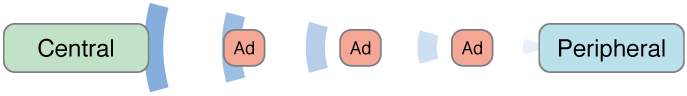
\includegraphics[width=0.65\textwidth]{images/AdvertisingAndDiscovery.png} 
    \caption{Advertising and discovery.}
    \end{center}
\end{figure}

\section{A peripheral, a service, a characteristic}

\begin{figure}[h]
    \begin{center}
    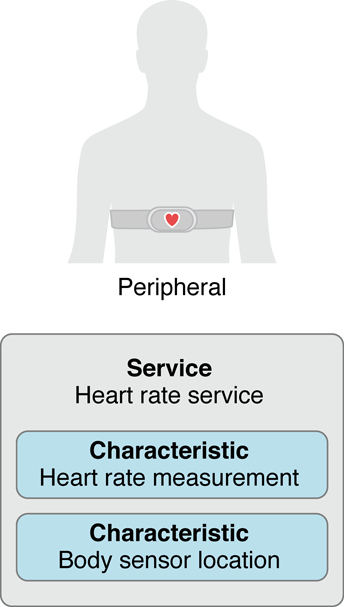
\includegraphics[height=0.25\textheight]{images/CBPeripheralData.png} 
    \caption{A remote peripheral’s tree of services and characteristics.}
    \end{center}
\end{figure}

\begin{figure}[h]
    \begin{center}
    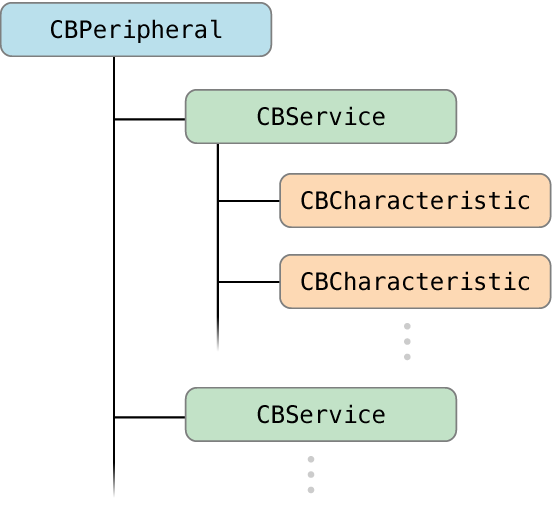
\includegraphics[height=0.25\textheight]{images/TreeOfServicesAndCharacteristics.png} 
    \caption{A peripheral’s service and characteristics.}
    \end{center}
\end{figure}

\begin{figure}[h]
    \begin{center}
    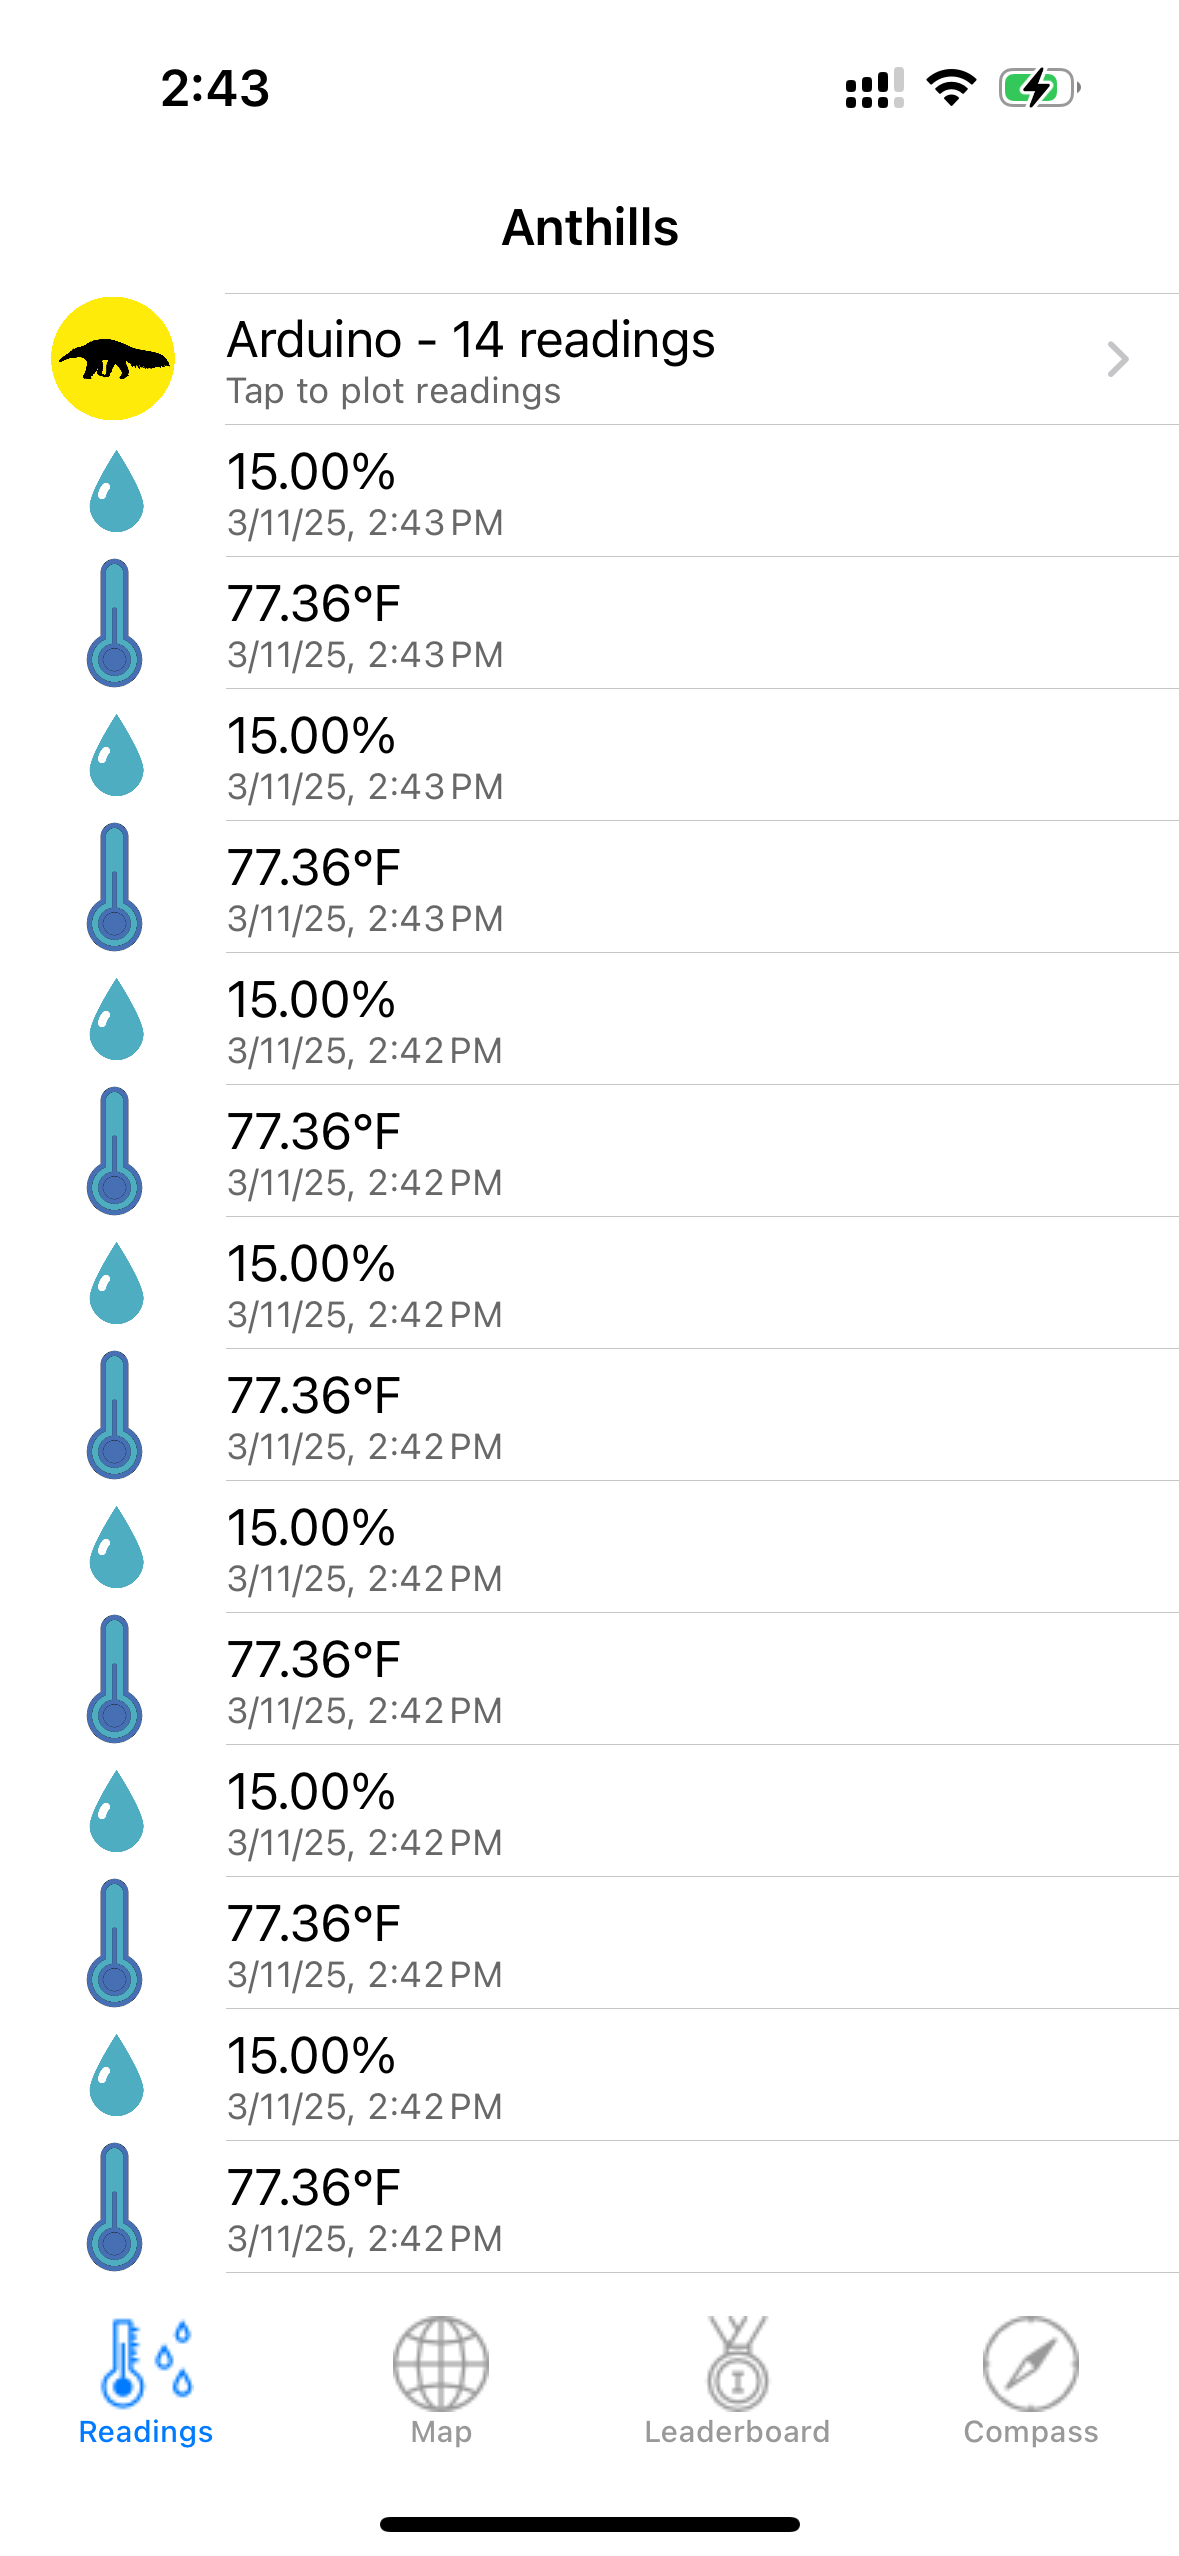
\includegraphics[height=0.35\textheight]{images/anthill.png} 
    \caption{Anthill discovered and transmitting data to client device.}
    \end{center}
\end{figure}


\section{Time Spent} 

Time spent:

% list of items:
\begin{itemize}
  \item Section 1: = 2 hour
  \item Section 2: = 1 hour
\end{itemize}


\end{document}

